\documentclass[journal]{vgtc}               % final (journal style)
%\documentclass[review,journal]{vgtc}         % review (journal style)
%\documentclass[widereview]{vgtc}             % wide-spaced review
%\documentclass[preprint,journal]{vgtc}       % preprint (journal style)

%% Uncomment one of the lines above depending on where your paper is
%% in the conference process. ``review'' and ``widereview'' are for review
%% submission, ``preprint'' is for pre-publication, and the final version
%% doesn't use a specific qualifier.

%% Please use one of the ``review'' options in combination with the
%% assigned online id (see below) ONLY if your paper uses a double blind
%% review process. Some conferences, like IEEE Vis and InfoVis, have NOT
%% in the past.

%% Please note that the use of figures other than the optional teaser is not permitted on the first page
%% of the journal version.  Figures should begin on the second page and be
%% in CMYK or Grey scale format, otherwise, colour shifting may occur
%% during the printing process.  Papers submitted with figures other than the optional teaser on the
%% first page will be refused. Also, the teaser figure should only have the
%% width of the abstract as the template enforces it.

%% These few lines make a distinction between latex and pdflatex calls and they
%% bring in essential packages for graphics and font handling.
%% Note that due to the \DeclareGraphicsExtensions{} call it is no longer necessary
%% to provide the the path and extension of a graphics file:
%% 
\includegraphics{diamondrule} is completely sufficient.
%%
\ifpdf%                                % if we use pdflatex
  \pdfoutput=1\relax                   % create PDFs from pdfLaTeX
  \pdfcompresslevel=9                  % PDF Compression
  \pdfoptionpdfminorversion=7          % create PDF 1.7
  \ExecuteOptions{pdftex}
  \usepackage{graphicx}                % allow us to embed graphics files
  \DeclareGraphicsExtensions{.pdf,.png,.jpg,.jpeg} % for pdflatex we expect .pdf, .png, or .jpg files
\else%                                 % else we use pure latex
  \ExecuteOptions{dvips}
  \usepackage{graphicx}                % allow us to embed graphics files
  \DeclareGraphicsExtensions{.eps}     % for pure latex we expect eps files
\fi%

%% it is recomended to use ``\autoref{sec:bla}'' instead of ``Fig.~\ref{sec:bla}''
\graphicspath{{figures/}{pictures/}{images/}{./}} % where to search for the images

\usepackage{microtype}                 % use micro-typography (slightly more compact, better to read)
\PassOptionsToPackage{warn}{textcomp}  % to address font issues with \textrightarrow
\usepackage{textcomp}                  % use better special symbols
\usepackage{mathptmx}                  % use matching math font
\usepackage{times}                     % we use Times as the main font
\renewcommand*\ttdefault{txtt}         % a nicer typewriter font
\usepackage{cite}                      % needed to automatically sort the references
\usepackage{tabu}                      % only used for the table example
\usepackage{booktabs}                  % only used for the table example
%% We encourage the use of mathptmx for consistent usage of times font
%% throughout the proceedings. However, if you encounter conflicts
%% with other math-related packages, you may want to disable it.

%% In preprint mode you may define your own headline.
%\preprinttext{To appear in IEEE Transactions on Visualization and Computer Graphics.}

%% If you are submitting a paper to a conference for review with a double
%% blind reviewing process, please replace the value ``0'' below with your
%% OnlineID. Otherwise, you may safely leave it at ``0''.
\onlineid{0}

%% declare the category of your paper, only shown in review mode
\vgtccategory{Research}
%% please declare the paper type of your paper to help reviewers, only shown in review mode
%% choices:
%% * algorithm/technique
%% * application/design study
%% * evaluation
%% * system
%% * theory/model
\vgtcpapertype{please specify}

%%%%%%%%%%%%%%%%%%%%%%%%%%%%%%%%%%%%%%%%%%%%%%%%%%%%%%%%%%%%%%%%
%%%%%%%%%%%%%%%%%%%%%%%%%%% TITLE %%%%%%%%%%%%%%%%%%%%%%%%%%%%%%
%%%%%%%%%%%%%%%%%%%%%%%%%%%%%%%%%%%%%%%%%%%%%%%%%%%%%%%%%%%%%%%%

%% Paper title.
\title{Applying signal processing strategies to attenuate Flame Detector analogue noise generated by GHz frequency interference}

%% This is how authors are specified in the journal style

%% indicate IEEE Member or Student Member in form indicated below
\author{Daniel Sikar - INM433 Individual Coursework - PT1 MSc Data Science}
\authorfooter{
%% insert punctuation at end of each item
\item
 Daniel Sikar - City University of London. E-mail: daniel.sikar@city.ac.uk
}

%%%%%%%%%%%%%%%%%%%%%%%%%%%%%%%%%%%%%%%%%%%%%%%%%%%%%%%%%%%%%%%%
%%%%%%%%%%%%%%%%%%%%%%%%%% ABSTRACT %%%%%%%%%%%%%%%%%%%%%%%%%%%%
%%%%%%%%%%%%%%%%%%%%%%%%%%%%%%%%%%%%%%%%%%%%%%%%%%%%%%%%%%%%%%%%

%% \input{INM430-final-report-0.5-abstract.tex}

%%%%%%%%%%%%%%%%%%%%%%%%%%%%%%%%%%%%%%%%%%%%%%%%%%%%%%%%%%%%%%%%
%%%%%%%%%%%%%%%%%%%%%%%%%% KEYWORDS %%%%%%%%%%%%%%%%%%%%%%%%%%%%
%%%%%%%%%%%%%%%%%%%%%%%%%%%%%%%%%%%%%%%%%%%%%%%%%%%%%%%%%%%%%%%%

%% Keywords that describe your work. Will show as 'Index Terms' in journal
%% please capitalize first letter and insert punctuation after last keyword
\keywords{Signal processing, analogue noise, gigahertz frequency interference}

%% ACM Computing Classification System (CCS). 
%% See <http://www.acm.org/class/1998/> for details.
%% The ``\CCScat'' command takes four arguments.

\CCScatlist{ % not used in journal version
 \CCScat{K.6.1}{Management of Computing and Information Systems}%
{Project and People Management}{Life Cycle};
 \CCScat{K.7.m}{The Computing Profession}{Miscellaneous}{Ethics}
}

%% Uncomment below to include a teaser figure.
\teaser{
  \centering
  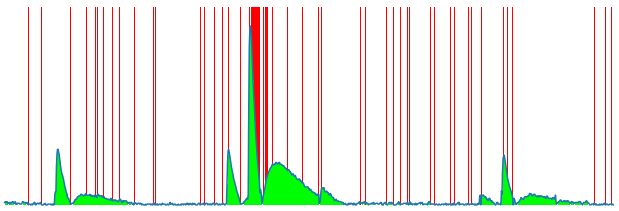
\includegraphics[width=\linewidth]{teaser.png}
 \caption{Plot showing distance function (blue), antiphase between channels (red) and area to be smoothed (green).}
	\label{fig:teaser}
}

%% Uncomment below to disable the manuscript note
\renewcommand{\manuscriptnotetxt}{}

%% Copyright space is enabled by default as required by guidelines.
%% It is disabled by the 'review' option or via the following command:
% \nocopyrightspace

\vgtcinsertpkg

%%%%%%%%%%%%%%%%%%%%%%%%%%%%%%%%%%%%%%%%%%%%%%%%%%%%%%%%%%%%%%%%
%%%%%%%%%%%%%%%%%%%%%% START OF THE PAPER %%%%%%%%%%%%%%%%%%%%%%
%%%%%%%%%%%%%%%%%%%%%%%%%%%%%%%%%%%%%%%%%%%%%%%%%%%%%%%%%%%%%%%%%

\begin{document}

%% The ``\maketitle'' command must be the first command after the
%% ``\begin{document}'' command. It prepares and prints the title block.

%% the only exception to this rule is the \firstsection command

\firstsection{Introduction}

\maketitle

%%%%%%%%%%%%%%%%%%%%%%%%%%%%%%%%%%%%%%%%%%%%%%%%%%%%%%%%%%%%%%%%
%%%%%%%%%% MOTIVATION, DATA AND RESEARCH QUESTIONS %%%%%%%%%%%%%
%%%%%%%%%%%%%%%%%%%%%%%%%%%%%%%%%%%%%%%%%%%%%%%%%%%%%%%%%%%%%%%%

%% INTRODUCTION

This study if motivated by the need to investigate strategies to process signals subject to RF (radio frequency) interference, eliminating what may be interpreted as noise, while preserving the signal. We investigating in particular commercially available Flame Detectors, taking into consideration approval processes related to IEC61508 \cite{wiki:IEC61508} SIL (Safety Integrity Level) approvals, which provide certification, as required by the insurance sector, to ensure compliance.

The data analysed in this study consists of 28 log files generated by UUTs (units under test) in a certified testing facility, where the UUT is place in a chamber where it is subjected to RF interference. Tests last up till five minutes, with acquisitions made at 10ms intervals. Each acquisition comprising of the analogue-to-digital converted signals of 3 sensors; 2 being redundant flame detectors and 1 being a "guard" which detects \textit{blackbody radiation} \cite{Massoud:2005} and can be used to avoid false positives i.e. heat being incorrectly identified as a flame.

Each observation (log entry) consists of 6 bytes, one for the Flame A channel, one for the Flame B channel and one for the Guard Channel. The value being an unsigned byte, ranging from 0 to 255. The fourth byte consisting of two 4 unsigned bit values ranging from 0 to 15. These are the voltage references for the flame sensors. Byte 5 is not used and byte 6 consists of three flags (bit values), one unused bit value and a four bit rolling counter to ensure readings are continuous. 

The data is retrieved from the UUT internal storage as a plain text file, which each acquisition stored in hexadecimal format, which must be processed by converting each byte into a base 10 number, with further masking to retrieve flags and four bit values.

Once the data is presented in a familiar decimal format, the research questions we would like to ask is how do different signal processing strategies perform in attenuating noise? What metrics can be used to quantify noise and can the same metrics be used to determine the suitability of one strategy over another?


%%%%%%%%%%%%%%%%%%%%%%%%%%%%%%%%%%%%%%%%%%%%%%%%%%%%%%%%%%%%%%%%
%%%%%%%%%%%%%%%%% TASKS AND APPROACH %%%%%%%%%%%%%%%%%%%%%%%%%%%
%%%%%%%%%%%%%%%%%%%%%%%%%%%%%%%%%%%%%%%%%%%%%%%%%%%%%%%%%%%%%%%%

\section{Tasks and approach}

Of special importance to this study is the fact that of the 28 log files, \textit{Test45.log} was generated by a UUT exposed to a flame while subject to no RF interference, and this file should be our reference to characterise signal, while all remaining files were generated by UUTs exposed to RF interference and no flame, and should be our references to charaterise noise.

With that in mind, our tasks are:

\subsection{Feature engineering}

To proceed with the remaining tasks, a number of features need to be created first, based on Channel A and Channel B values for every log these involve

\begin{itemize}
    \item Log file name
    \item Channel 1 (flame a) raw data
    \item Channel 2 (flame b) raw data
    \item Channel 1 normalised data
    \item Channel 2 normalised data
    \item Normalised distance function
    \item Antiphase function
    \item Normalised correlation coefficient
    \item Filtered (Savitzy-Golay filter) channel 1 normalised data
    \item Filtered (Savitzy-Golay filter) channel 2 normalised data
    \item Filtered distance function
    \item Filtered antiphase function
    \item Filtered correlation coefficient
    \item Interpolated channel 1 normalised data
    \item Interpolated channel 2 normalised data
    \item Interpolated distance function
    \item Interpolated antiphase function
    \item Interpolated correlation coefficient
\end{itemize}

\subsection{Characterising signal and noise}

To characterise noise and signal we shall plot Flame A and Flame B values for our flame reference file, compared to another file then compare plots.

\subsection{Antiphase function}

The computational method for our antiphase function can be expressed by:

$$  A \Rightarrow \frac{\Delta Fa}{\Delta Fb}<0$$
where
$$ \Delta Fa = Fa{_i}-Fa{_{i-1}}, \Delta Fb = Fb{_i}-Fb{_{i-1}}, \forall i > 1 $$

The sign of delta ratios indicating phase (positive) or antiphase (negative).

Our visual method is to plot detected antiphase together the time series for the flame channels.

\subsection{Distance function}

We use a distance function defined as:

$$ Fd = |Nfa - Nfb| $$

Where Fd is the absolute difference between channels a and b. Visually distance between channels is displayed as a plot. 

\subsection{Correlation coefficient}

We extract a correlation coefficient \textbf{between} channel 1 (x) and channel 2 (y) - it is important to noticed here that we are using the correlation coefficient to determine how close the signals are to each other and not how one might be affecting the other.

$$ r =\frac{\sum ^n _{i=1}(x_i - \bar{x})(y_i - \bar{y})}{\sqrt{\sum ^n _{i=1}(x_i - \bar{x})^2} \sqrt{\sum ^n _{i=1}(y_i - \bar{y})^2}} $$

We will use the output to have all coefficients in tabular form for comparison, as well as headers for sample plots.

\subsection{Savistzky-Golay filter}

We use a Savitzky-Golay filter \cite{Savitzky:1964} defined as:

$$ Y_j= \sum _{i=\tfrac{1-m}2}^{\tfrac{m-1}2}C_i\, y_{j+i},\qquad  \frac{m-1}{2} \le j \le n-\frac{m-1}{2} $$

where x is an independent variable and yj is an observed value. Note we are applying the filter \textbf{independently} to each of the channels a and b signals, to then obtain a correlation coefficients as well as additional engineered features.

This will used to generate data for linear regression plots as well as correlation coefficients.

\subsection{Linear Interpolation}

We use a linear interpolation algorithm, for all observations where the distance between channels, at the observation index, is greater than a threshold \textit{t}, defined as:

$$ y = \frac{y_0(x_1-x)+y_1(x-x_0)}{x_1-x_0} , \forall Fd > t $$

Notice this is also applied, as the previous filter, on a per-channel basis, x being the independent and y being the dependent variable.
This will used to generate data for linear regression plots as well as correlation coefficients. 

NB all normalisation is done using minimum and maximum values scaled to byte values (0-255):

$$ z{_i}=\frac{x{_i}-min}{max-min} , max-min \neq 0 $$

%%%%%%%%%%%%%%%%%%%%%%%%%%%%%%%%%%%%%%%%%%%%%%%%%%%%%%%%%%%%%%%%
%%%%%%%%%%%%%%%%%%% ANALYTICAL STEPS %%%%%%%%%%%%%%%%%%%%%%%%%%%
%%%%%%%%%%%%%%%%%%%%%%%%%%%%%%%%%%%%%%%%%%%%%%%%%%%%%%%%%%%%%%%%

\section{Analytical steps}

Once all our engineered features have been generated from channel 1 and 2, for all log files, we can proceed with our analysis.
Our first step is to characterise noise and signal, so we plot a significant section of both, taken from \textit{Test45.log} and \textit{Test48.log}. Each plot consisting of a 12 second sample approximately. we plot the value of channel 1 (Flame A) in blue and (Flame b) in orange. 

We see from Fig. 2. that in our signal data, both channels are tightly coupled, and there could be a number of different markers to show this, correlation and distance being two possible choices. As a result channel 2 almost hides channel 1. The disturbance in the middle section being a barbecue lighter lit while the UUT was logging.

We then see from Fig. 3. that our noise data shows less overlap and greater distance between both channels, as well as antiphase, so these engineered features could be used charaterise noise. Both channels are mostly visible and both colours can be distinguished.

We now have visual markers for signal and noise, based on our computation. we are now equipped to create additional plots, where antiphase and distance can be added. Fig. 4. has the same plot as Fig. 2 with the added antiphase and distance functions, where it is clear that actual fire signal has no antiphase, the overall distance function being consistently at the lower end of the normalised byte scale. Both markers together can provide a good indication of where a noise attenuating scheme such as linear interpolation would be useful, as can be seen in Fig. 5. with distance and antiphase function plots together with noise. A next step in visualisation can be seen in Fig. 6. where the channels 1 and 2 are removed from the plot, and the area under the distance function is highlighted in green. We now, using this scheme, apply linear interpolation to minimise areas under the function, obtaining data to generate plots and lines of best fit, together with correlation coefficients. Nothing again that we are not interested in the value of $ r^2 $, as correlation coefficient is used as a proxy for distance.
The stopping condition for our linear interpolation algorithm being the best threshold \textit{t}, preserving signal while eliminating most of the noise.
Visual analytics motivated the search for a second attenuation algorithm (linear interpolation), as visually is was clear that mearly smoothing a signal would not minimise the distance or antiphase functions.

We created 3 series of 6 sample plots for the original normalised data, Savistzky-Golay filtered data and Linear Interpolation smoothed data, in Fig. 7., Fig. 8. and Fig. 9. respectively, showing best lines of fit, together with correlation coefficients, these should help inform which schemes work best.

Note no channel 1 and channel 2 plots are shown here for the Savistzky-Golay filter or linear interpolation filter, for the sake of keeping a good balance between text and images. It is worth mentioned that the stopping condition for the Savitzky-Golay filter is found based on experimentations with the window length and polynomial order, and are an artifact of previous work \cite{Sikar:INM430}. Note these values where obtained empirically, and not though a specific computational technique.

The last piece of computation and visual methods is the more traditional Table 1., with an asterisk denoting which scheme provided the highest correlation coefficient, minimising the distance between channel 1 and channel 2 and as a consequence, attenuating the noise. 

\begin{figure}[tb]
 \centering % avoid the use of \begin{center}...\end{center} and use \centering instead (more compact)
 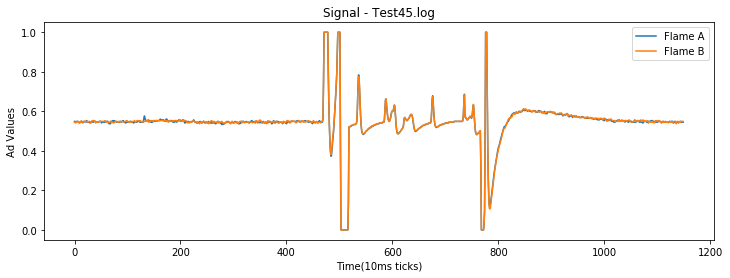
\includegraphics[width=\columnwidth]{pictures/05-signal.png}
 \caption{Characterising noise and signal - Signal data, generated by waving a barbecue lighter in front of UUT}
 \label{fig:sample}
\end{figure}



\begin{figure}[tb]
 \centering % avoid the use of \begin{center}...\end{center} and use \centering instead (more compact)
 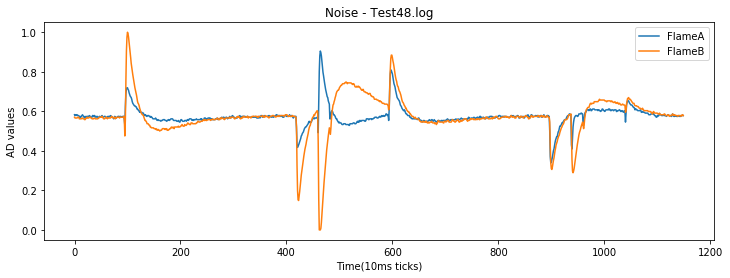
\includegraphics[width=\columnwidth]{pictures/04-noise.png}
 \caption{Characterising noise and signal - Noise data, generated by subjecting UUT to RF interference}
 \label{fig:sample}
\end{figure}

\begin{figure}[tb]
 \centering % avoid the use of \begin{center}...\end{center} and use \centering instead (more compact)
 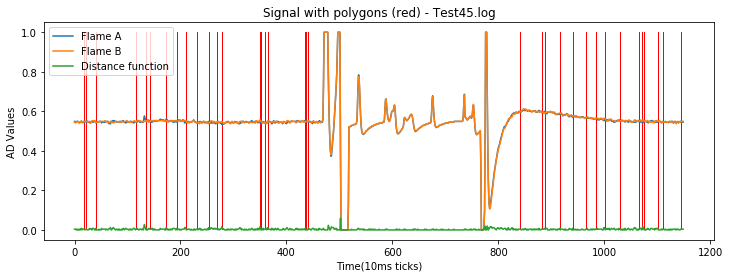
\includegraphics[width=\columnwidth]{pictures/06-signal-antiphase-distance.png}
 \caption{Signal plot with distance and antiphase functions.}
 \label{fig:sample}
\end{figure}

\begin{figure}[tb]
 \centering % avoid the use of \begin{center}...\end{center} and use \centering instead (more compact)
 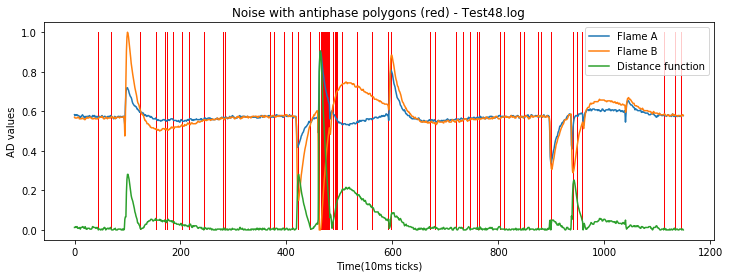
\includegraphics[width=\columnwidth]{pictures/07-noise-antiphase-distance.png}
 \caption{Noise plot with distance and antiphase functions.}
 \label{fig:sample}
\end{figure}

\begin{figure}[tb]
 \centering % avoid the use of \begin{center}...\end{center} and use \centering instead (more compact)
 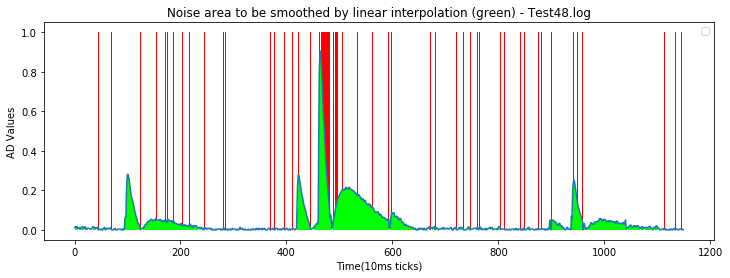
\includegraphics[width=\columnwidth]{pictures/08-noise-linear-interpolation-smoothing.png}
 \caption{Noise plot with area to be smoothed by linear interpolation.}
 \label{fig:sample}
\end{figure}

\begin{figure}[tb]
 \centering % avoid the use of \begin{center}...\end{center} and use \centering instead (more compact)
 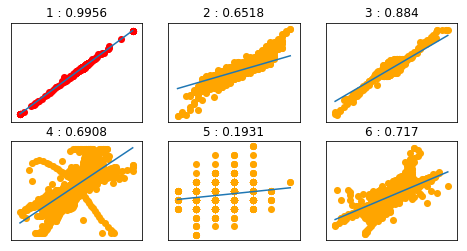
\includegraphics[width=\columnwidth]{pictures/01-raw-linear-regression.png}
 \caption{Linear Regression for 6 sample log files, with lines of best fit and correlation coefficients for normalised data. Top left plot (1) is real fire data, remaining plots contain interference data}
 \label{fig:sample}
\end{figure}

\begin{figure}[tb]
 \centering % avoid the use of \begin{center}...\end{center} and use \centering instead (more compact)
 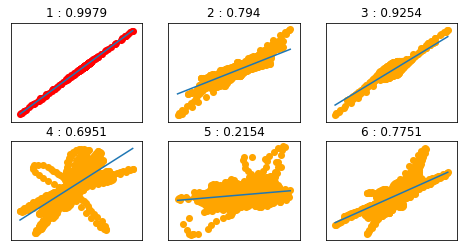
\includegraphics[width=\columnwidth]{pictures/02-sg-linear-regression.png}
 \caption{Linear Regression for 6 sample log files, with lines of best fit and correlation coefficients for Savitzky-Golay filtered data. Top left plot (1) is real fire data, remaining plots contain interference data.}
 \label{fig:sample}
\end{figure}

\begin{figure}[tb]
 \centering % avoid the use of \begin{center}...\end{center} and use \centering instead (more compact)
 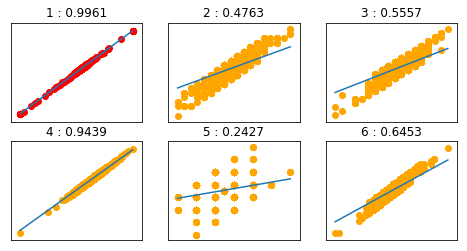
\includegraphics[width=\columnwidth]{pictures/03-li-linear-regression.png}
 \caption{Linear Regression for 6 sample log files, with lines of best fit and correlation coefficients for linear interpolation smoothed data. Top left plot (1) is real fire data, remaining plots contain interference data.}
 \label{fig:sample}
\end{figure}



%%%%%%%%%%%%%%%%%%%%%%%%%%%%%%%%%%%%%%%%%%%%%%%%%%%%%%%%%%%%%%%%
%%%%%%%%%%%%%%%%%%%%%%%% FINDINGS %%%%%%%%%%%%%%%%%%%%%%%%%%%%%%
%%%%%%%%%%%%%%%%%%%%%%%%%%%%%%%%%%%%%%%%%%%%%%%%%%%%%%%%%%%%%%%%

\section{Findings}

We found metrics to characterise as well as distinguish signal from noise and provide attenuation boundaries for the linear interpolation scheme.

We applied two signal processing strategies to attenuate noise, and found that both SG (Savitzky-Golay) and LI (Linear Interpolation) increased correlation coefficients in most cases, though in some cases such as Test52.log SG decreased the correlation coefficient while in cases such as Test46.log, LI decresed the correlation, coefficient. On the whole SG performed better than LI.

We found that signal had low distance functions, while noise had high distance functions in the presence of antiphase, as both signals are travelling in opposite directions.

Distance turned out to be a good proxy for noise, with the higher values being directly proportional to higher noise, i.e. channels 1 and 2 far from each other, while lower values mean lower noise and consequently, higher signal.

Antiphase was also an interesting marker as it seems to occur frequently though was not see in the presence of signal.

A key finding was that both SG and LI actually improved correlation coefficients for our reference signal file Test45.log

Table \ref{table:kysymys} on page \pageref{table:kysymys} refers to the correlation coefficients, where CC is the original, SGCC is the filtered and ICC is the interpolated data correlation coefficient between channels a and b. Asterisks denote highest correlation coefficient in row.

We established that a large proportion of the variation can be explained by interference, when signals go into antiphase, increasing the distance between values.

We found that applying the Savistzky-Golay filter decreased the distance, in turn decreasing noise. Contrary to expectation, we found that no single scheme worked best as shown in Table 1, where some correlation coefficients are improved by filtering while others are improved by linear interpolation.

One research question that could not be answered was how metrics obtained (as described in 2.1) could be used to determine the suitability of one strategy over another. As seen in Table 1. SG and LI perform different and it would have been good to determine the reasons for this difference, predicting ahead of time, when to best use one or the other. We expand more on this topic in the next section.

\begin{table}[]
\centering
\begin{tabular}{|l|l|l|l|}
\hline
\multicolumn{4}{|l|}{Original, filtered and interpolated data} \\ \hline
Log file  &  CC & SGCC & ICC \\ \hline
Test45.log & 0.9956 & 0.9979 * & 0.9961 \\ \hline
Test46.log & 0.6518 & 0.7940 * & 0.4763 \\ \hline
Test47.log & 0.8840 & 0.9254 * & 0.5557 \\ \hline
Test48.log & 0.6908 & 0.6951 & 0.9439 * \\ \hline
Test49.log & 0.1931 & 0.2154 & 0.2427 * \\ \hline
Test50.log & 0.7170 & 0.7751 * & 0.6453 \\ \hline
Test51.log & 0.8739 & 0.8827 & 0.9927 * \\ \hline
Test52.log & 0.3417 & 0.3394 & 0.9083 * \\ \hline
Test53.log & 0.9146 & 0.9220 & 0.9914 * \\ \hline
Test54.log & 0.9172 & 0.9275 & 0.9771 * \\ \hline
Test55.log & 0.8123 & 0.8739 * & 0.5765 \\ \hline
Test56.log & 0.8891 & 0.9020 * & 0.8978 \\ \hline
Test57.log & 0.3361 & 0.3370 & 0.7804 * \\ \hline
Test58.log & 0.2004 & 0.2245 & 0.2729 * \\ \hline
Test59.log & 0.3922 & 0.5423 * & 0.3553 \\ \hline
Test60.log & 0.4395 & 0.5177 * & 0.4593 \\ \hline
Test61.log & 0.1974 & 0.1916 & 0.2653 * \\ \hline
Test62.log & 0.4155 & 0.5919 * & 0.4111 \\ \hline
Test63.log & 0.5986 & 0.7438 * & 0.4770 \\ \hline
Test64.log & 0.5219 & 0.7022 * & 0.3897 \\ \hline
Test65.log & 0.2200 & 0.2588 & 0.2898 * \\ \hline
Test66.log & 0.3489 & 0.4134 * & 0.3954 \\ \hline
Test67.log & 0.8746 & 0.8895 * & 0.7683 \\ \hline
Test68.log & 0.7765 & 0.7922 * & 0.7790 \\ \hline
Test69.log & 0.2566 & 0.2577 & 0.9030 * \\ \hline
Test70.log & 0.4387 & 0.6178 * & 0.4610 \\ \hline
Test71.log & 0.6141 & 0.7820 * & 0.4476 \\ \hline
Test72.log & 0.7652 & 0.7695 & 0.9456 * \\ \hline

\end{tabular}
\caption{Correlation coefficients}
\label{table:kysymys}
\end{table}


%%%%%%%%%%%%%%%%%%%%%%%%%%%%%%%%%%%%%%%%%%%%%%%%%%%%%%%%%%%%%%%%
%%%%%%%%%%%%%%%%%%% CRITICAL REFLECTION %%%%%%%%%%%%%%%%%%%%%%%%
%%%%%%%%%%%%%%%%%%%%%%%%%%%%%%%%%%%%%%%%%%%%%%%%%%%%%%%%%%%%%%%%

\section{Critical reflection}

The results of this study have shown that, from a noise filtering perspective, different filters may offer better performance for a set of similar signal types, in other words, we have seen that for some logs, a moving window filter, applied to each channel individually, generated better correlation between both channels.

Visual analytics helped characterise signal and noise and therefore to determine differences. Once additional features had been engineered and visualised, it was implied that linear interpolation might provide good results in eliminating noise, and ultimately increasing the correlation between the two channels.

The approach suggested in this study could be applied to other equipment subject to IEC 61508 approvals, as any analogue to digital conversion process subject to interference would be likely to present the same noise. The distinguishing factor being the peculiarity of the flame detector under test presenting two flame detectors and the approach of bringing both signals in line with each other. Any equipment with redundant sensors could benefit from such approach, probably still within the signal processing domain, as redundancy seems to be a peculiarity on most systems with some degree of realtime computing \cite{Kane:1992}.

The antiphase function would have benefited from a window approach, whereby a sequence is taken instead of an observation index in relation to the preceding index. The antiphase plots, although illustrative were somewhat counterintuitive, as areas that were visualise showing channels 1 and two travelling in opposite direction where not showing antiphase polygon highlights. This may be explained in part because the plots are very dense, many data points having to be represented as a single pixel, so perhaps if this is a shortcoming of the method, the display or both could be a subject for future studies.

The distance function visually worked quite well once it was highlighted though the actual linear interpolation algorithm should take both distance and antiphase into account though in this study, in the end, only distance was used while antiphase was not used to determine which areas should be smoothed by linear interpolation. In future an more robust algorithm should account for both.

The Savistsky-Golay filter provided improved correlation coefficients between channels, once the signals had been filtered via this method. Ideally the window length and polynomial order should be optimised on a per section basis, with a look ahead scheme with a buffered output, where a decision could be made about what the optimal parameters would be.

The same applies to Linear Interpolation, where a buffer scheme could provide a delay in which to decide which should be used, filtering or interpolation as, we have noticed, both have optimal performing instances, though this study could not conclude what those aspects could be.

On the whole, this study achieved its goal in quantifying signal processing strategy performance in attenuating noise and in establishing what metrics can be used. It did so by the use of computational and visual techniques, to process data and generate plots, to the inform decisions\cite{Sikar:INM433} . In was not able to determine at this stage the suitability of one strategy over another at this stage.

%%%%%%%%%%%%%%%%%%%%%%%%%%%%%%%%%%%%%%%%%%%%%%%%%%%%%%%%%%%%%%%%
%%%%%%%%%%%%%%%%%%%%%% ACKNOWLEDGEMENTS %%%%%%%%%%%%%%%%%%%%%%%%
%%%%%%%%%%%%%%%%%%%%%%%%%%%%%%%%%%%%%%%%%%%%%%%%%%%%%%%%%%%%%%%%

\acknowledgments{
We wish to thank Gennady and Natalia Andrienko, Alex Galkin, Aidan Slingsby and Abi Sowri for their guidance and support.}

%\bibliographystyle{abbrv}
\bibliographystyle{abbrv-doi}
%\bibliographystyle{abbrv-doi-narrow}
%\bibliographystyle{abbrv-doi-hyperref}
%\bibliographystyle{abbrv-doi-hyperref-narrow}

\bibliography{INM433-7-references}

\end{document}

